\section{The classical Black Hole Area Theorem}
\label{sec:classical-bh-area}

%todo; scrivere che BH non possono separarsi
Our statement of the Black Hole Area Theorem comes from \cite{wald2010general} (theorem \(12.2.6\)):
%todo: restate the tehorem only using \mathscr{H}, non serve distinguere tra 1 e 2 secondo me.
\begin{theorem}[Black Hole Area Theorem]
	\label{th:classical-bh-area}
	Let \((M, g_{\mu\nu})\) be a strongly asymptotically predictable spacetime satisfying \(R_{\mu\nu}U^{\mu}U^{\nu} \ge 0\) for all null vectors \(U^{\mu}\) (\emph{null convergence condition}). Let \(\Sigma_1\) and \(\Sigma_2\) be spacelike Cauchy surfaces for the globally hyperbolic region \(\tilde{V}\) such that \(\Sigma_2 \subset I^+(\Sigma_1)\), and given \(H\) the event horizon we define
	\[
	\mathscr{H}_1 = H \cap \Sigma_1 \quad \quad \mathscr{H}_2 = H \cap \Sigma_2
	\]
	Then the area of \(\mathscr{H}_2\) is greater or equal than the area of \(\mathscr{H}_1\).
\end{theorem}

\begin{proof}
	This theorem is usually proven by showing, through a reductio ad absurdum, that the expansion \(\theta\) of the null geodesic generators of \(H\) is everywhere non-negative. Here we wish to follow a slightly different path, inspired by the index form methods, that makes use of another object, defined in section \ref{sec:submanifolds}: the mean curvature.
	
	Let \(\Sigma_1\) be any Cauchy hypersurface for \(\tilde{V}\) through a generic point \(p\in H\), and call \(\mathscr{H}_1 = H \cap \Sigma_1\), as above. Finally refer to \(\mathrm{H}^{\mu}\) as the mean normal curvature of \(\mathscr{H}_1\).
	The core of the proof is showing that, for the tangent field \(U^{\mu}\) of the null generators of the horizon \(H\), it holds everywhere that:
	\begin{equation}
	\label{eq:exp-null-generators}
		\mathrm{H}^{\mu}U_{\mu} \ge 0.
	\end{equation}
	By contradiction, suppose instead that \(\mathrm{H}^{\mu}U_{\mu} < 0\) at \(p\in \mathscr{H}_1\). We then want to extend the function \(\mathrm{H}^{\mu}U_{\mu}\) in a continuous way on \(\Sigma_1\) (at least in a neighborhood of \(\mathscr{H}_1\)). 
	
	In order to do that, take any deformation of \(\mathscr{H}_1\) outward on \(\Sigma_1\), say \(\mathscr{H}_1'\) and call \(K\) the closed region in \(\Sigma_1\) between \(\mathscr{H}_1\) and \(\mathscr{H}_1'\); the boundary of its future \(\partial J^+(K)\) is a null hypersurface of codimension \(1\), and hence comes with its own null generators, with tangent field \(U'^{\mu}\) (see figure \ref{fig:extension-area-theorem}). This allows us to define the function in \(p' \in\mathscr{H}_1'\) as simply the contraction 
	\(\mathrm{H}'^{\mu}U'_{\mu}\) (with \(\mathrm{H}'^{\mu}\) mean normal curvature of \(\mathscr{H}_1'\)). Different deformations of \(\mathscr{H}_1\) may give different extensions, but that's not important, since we only need that there exists one so that the extension is smooth.
	
	\begin{figure}
		\centering
		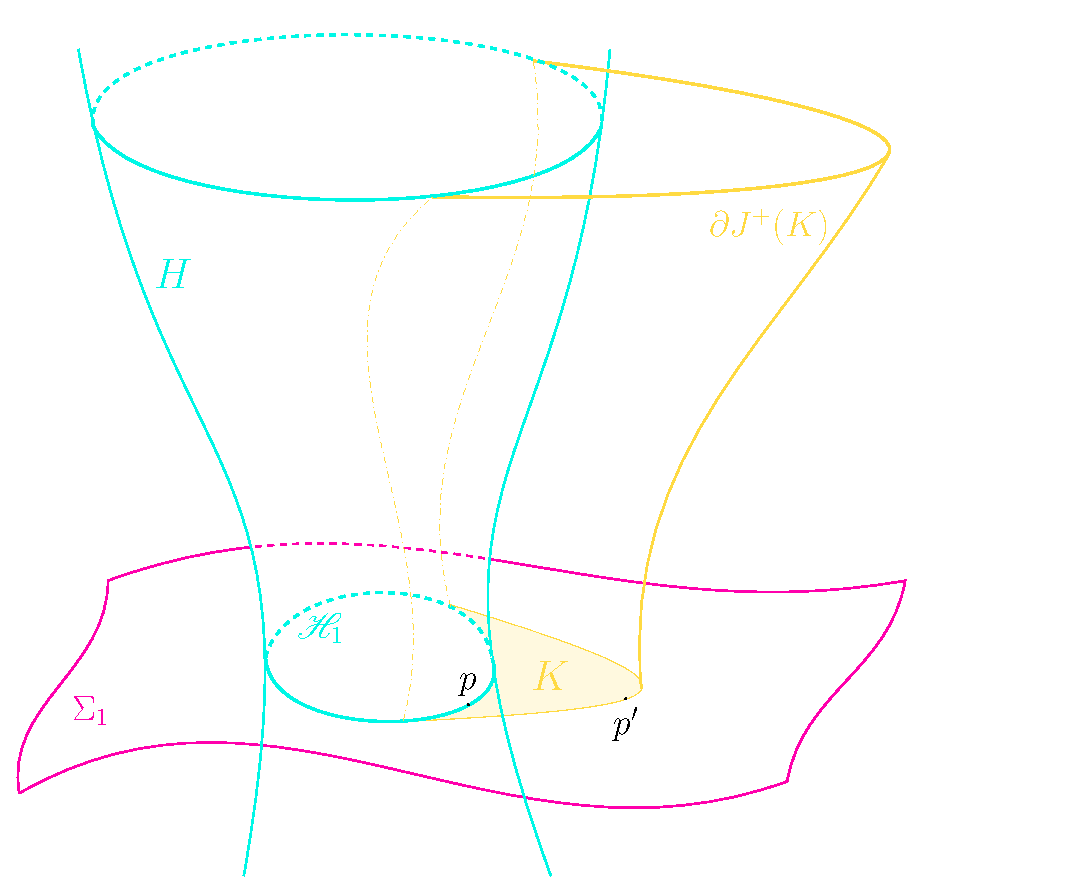
\includegraphics[scale=0.8]{Immagini/extension-area-theorem/extension-area-theorem.pdf}
		\caption[]{schematic representation about how to construct the extension of the function \(\mathrm{H}^{\mu}U_{\mu}\).}
		\label{fig:extension-area-theorem}
	\end{figure}
	\begin{SCfigure}
		\centering
		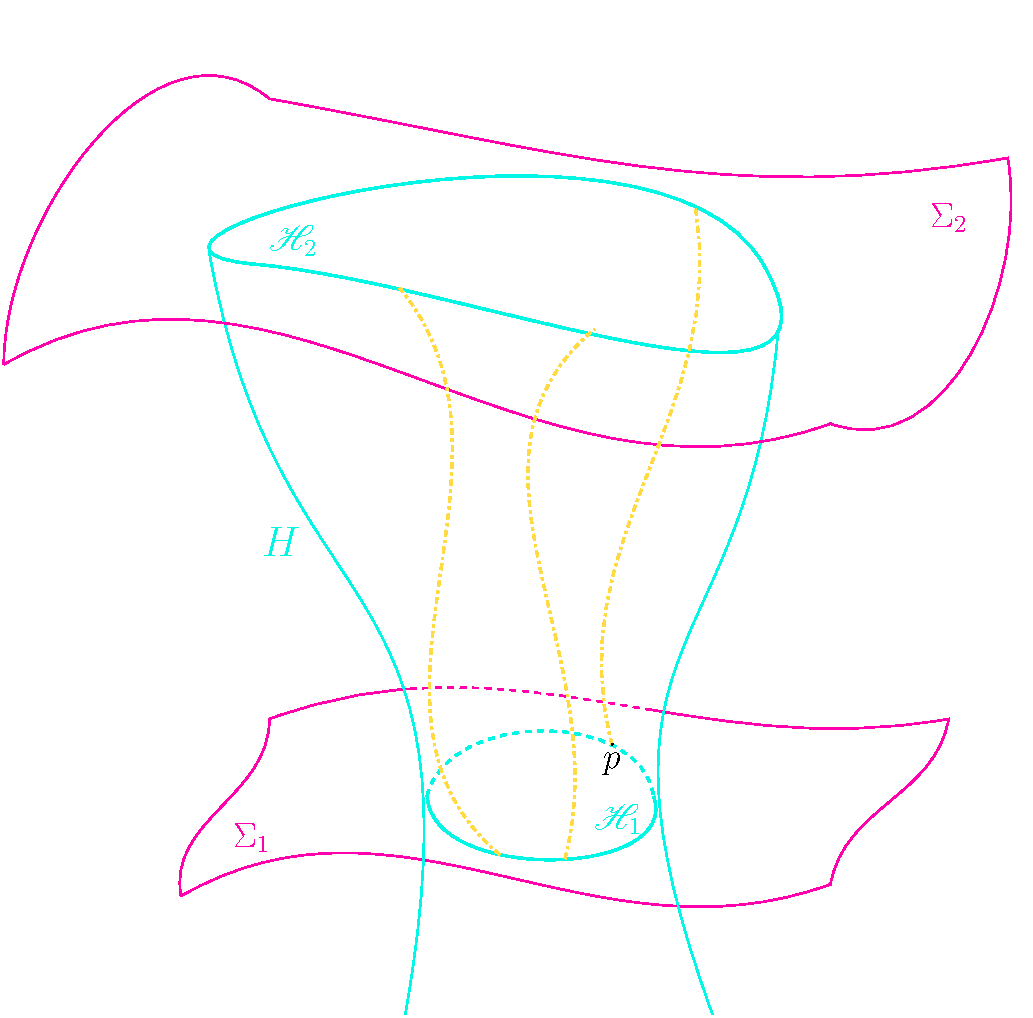
\includegraphics[scale=0.4]{Immagini/flow-generators/flow-generators.pdf}
		\caption[]{the flow along the null generators of the horizon maps \(\mathscr{H}_1\) into (a part of) \(\mathscr{H}_2\).}
		\label{fig:flow-generators}
	\end{SCfigure}
	Given that extension, it exists a neighborhood of \(p\) in which \(\mathrm{H}^{\mu}U_{\mu}(p) < 0\), we can pick a deformation \(\mathscr{H}_1\) outward on \(\Sigma_1\), to \(\mathscr{H}_1'\), such that
	\[
	\begin{cases}
	J^-(\mathscr{I}^+) \cap \mathscr{H}_1' \neq \emptyset; \\
	\mathrm{H}^{\mu}U'_{\mu} < 0 \text{ everywhere on } 	J^-(\mathscr{I}^+) \cap \mathscr{H}_1'
	\end{cases}
	\]
	
	Pick now a point \(q \in \mathscr{I}^+ \cap \partial J^+(K)\):  (\VS{This exists for sth similar to 12.2.6 of Wald})
	the null geodesic generator through \(q\) will meet \(\mathscr{H}_1'\) orthogonally because of \ref{prop:global-existence} and \ref{prop:perp-critical-gamma}; however in \(p' = \gamma \cap \mathscr{H}_1'\) \(U_{\mu}\mathrm{H}^{\mu} < 0\), so by proposition \ref{prop:fp-criteria} we know that a focal point to \(\mathscr{H}_1'\) must develop on \(\gamma\) before reaching \(q\). In fact, it is enough to choose \(f = 1 - \frac{\lambda}{\ell}\), with \(\lambda\) affine parameter such that:
	\[
	\begin{cases}
	\hat{\mathrm{H}}^{\mu}U_{\mu} = 1 \\
	\gamma(\lambda = 0) = p' \\
	\ell \ge  \frac{1}{\vert U_{\mu}\mathrm{H}^{\mu} \vert}
	\end{cases}
	\]
	and 
	{\small
	\[
	\int_{0}^{\ell} \big((n -2)(\nabla_Uf)^2 - f^2R_{\mu\nu}U^{\mu}U^{\nu} \big)d\lambda\le 
	\frac{n -2}{\ell} \le -(n -2) U_{\mu} \mathrm{H}^{\mu} =
	-(n -2) g(f^2 U, \mathrm{H})\Big\vert_{p},
	\]}
	This is impossible, because the null generator cannot contain any focal point, and hence 
	\[
	\forall p \in H \quad \mathrm{H}^{\mu}U_{\mu}(p) \ge 0.
	\]
		
	To conclude, it is enough to observe that each \(p\in \mathscr{H}_1\) lies on a null generator \(\gamma\) contained in \(H\). As \(\Sigma_2\) is a Cauchy hypersurface as well, \(\gamma\) must intersect \(\Sigma_2\) in a point \(q \in \mathscr{H}_2\). Then, the flow along null generators maps \(\mathscr{H}_1\) into a portion of \(\mathscr{H}_2\).
	
	But we know that under deformation along the flow of a vector field, the area of a submanifold evolves as \ref{eq:variation-area}, so:
	\begin{equation*}
		\delta_U\mathcal{A}_{\mathscr{H}_1} = \int_{\mathscr{H}_1} \mathrm{H}^{\mu}(p)U_{\mu} \ge 0
	\end{equation*}
	which is telling us that when we modify \(\mathscr{H}_1\) along the flow of the null generators the area of \(\mathscr{H}_1\) can never decrease.
\end{proof}

\section{The damped Averaged Null Energy Condition -- dANEC}
In section \ref{sec:classical-bh-area} we proved the black holes area theorem under classical hypothesis. As discussed in %todo: scrivi intro a energy conditions e metti una ref
the Null Energy Conditions is violated by any sort of quantum fields, while we wonder in what cases - if any - the theorem can be extended in a semiclassical regime.

One first attempt is obtained replacing the null energy conditions with its damped version; this result was already obtained by Lesourd in \cite{lesourd2018remark}, where it was used the Raychaudhuri's equation once again, while here we would like to propose an alternative proof, in the same spirit of theorem \ref{th:classical-bh-area}.
\begin{definition}
	A spacetime satisfies the \emph{damped averaged null energy condition} if along each future complete null geodesic \(\gamma\), affinely parametrized by \(\lambda\), there exists a non-negative constant \(c\ge 0\) such that:
	\[
	\liminf\limits_{\Lambda\rightarrow \infty} \int_{0}^{\Lambda} e^{-ct}R_{\mu\nu}U^{\mu}U^{\nu}d\lambda - \frac{c}{2} > 0
	\]
	where \(U^{\mu}\) is \(\gamma\)'s tangent field.
\end{definition}

The statement of the theorem is the same as \ref{th:classical-bh-area}, but replacing the Null convergence condition with dANEC; the proof is pretty similar as well but this time we will need to choose a different trial function when using proposition \ref{prop:fp-criteria}.
\begin{proof}
	Define \(\mathscr{H}_1\), and consider \(U_{\mu}\mathrm{H}^{\mu}\) exactly as in \ref{th:classical-bh-area}. Again we want to show that it needs to be \(U_{\mu}\mathrm{H}^{\mu} > 0\) everywhere on the horizon. In order to do it, by contradiction, assume there exists \(p\in \mathscr{H}_1\) for which this doesn't hold, and construct the extension \(U'_{\mu}\mathrm{H}'^{\mu}\) in a neighborhood of \(p\) in the same way as before.
	Now, pick \(f = e^{-c\frac{\lambda}{2}}\): the left hand side of \ref{eq:fp-criteria} in \(n = 4\) dimensions becomes:
	\[
	\int_{0}^{+\infty} (n-2)\frac{c^2}{4} e^{-c\lambda} - e^{-ct}R_{\mu\nu}U^{\mu}U^{\nu}d\lambda = \frac{c}{2} - \int_{0}^{+\infty} e^{-ct}R_{\mu\nu}U^{\mu}U^{\nu}d\lambda 
	\]
	which is negative, for the assumption of dANEC.
	Instead, \(U'_{\mu}\mathrm{H}'^{\mu} < 0 \) implies
	\[
	-(n - 2)U'_{\mu}\mathrm{H}'^{\mu} > 0.
	\]
	From this it follows that \ref{eq:fp-criteria} holds, and hence  a focal point is formed along \(\gamma\), which is, again, absurd. 
	
	By this contradiction we have that along the null generators \(U_{\mu}\mathrm{H}^{\mu} > 0\), and the conclusion is reached exactly ad in \ref{th:classical-bh-area}.
\end{proof}

Assuming the dANEC we are still able to prove that the area cannot decrease: this is a signal that we are still working with a classical condition; we will now move forward to conditions that reach weaker conclusions and hopefully are derived from weaker conditions.

\section{The Sobolev condition}
In this section we will assume the validity of a different energy condition, that uses Sobolev norms, and that's why we call it \emph{Sobolev condition}.
This assumption is motivated by the work in section \(4\) of \cite{fewster2020new}, where an analogous condition is assumed in order to derive singularity theorems.

\begin{definition}
	We say that the \emph{Sobolev condition} is satisfied on a curve \(\gamma\), from a Cauchy surface \(\Sigma\) for a ``time'' \(\ell\), if there exixst some \(m\in \N\) and \(2\) non negative constants \(Q_0\) and \(Q_m\) such that, for any \(\frac{1}{2}-\)density \(f\) on \(\gamma\):
    \begin{equation}
        \label{eq:Sobolev-condition}
        \int_0^{\ell} f(\lambda)^2 R_{\mu\nu}U^{\mu}U^{\nu} \ge -Q_m(\gamma) \vert\vert f^{(m)}\vert\vert^2 - Q_0(\gamma) \vert\vert f\vert\vert^2;
    \end{equation}

	the affine parametrization is chosen so that \(\gamma(\lambda = 0) \in \Sigma\) and \(\hat{H}_{\mu}\frac{d\gamma^{\mu}}{d\lambda}\Big\vert_{\lambda = 0} \equiv 1\) (\(\hat{H}_{\mu}\) is the versor of the mean normal curvature of \(\Sigma\)) - we will refer to this as the \emph{standard} affine parametrization. Finally, \(\vert\vert \star \vert\vert\) denotes the standard norm in \(L^2(I)\).
\end{definition}

Such a condition has some useful consequences on the functional \(J_{\ell}[f] = \int_0^{\ell} (n - 2)(\nabla_Uf)^2 - f^2R_{\mu\nu}U^{\mu}U^{\nu}(\lambda) d\lambda \).
\begin{lemma}
	\label{lemma:J-sobolev-condition}
	Let 
	\begin{itemize}
		\item[\ding{99}] the Sobolev condition be satisfied on \(\gamma\), from \(\Sigma\) for a ``time'' \(\ell\);
 		 \item[\ding{99}] the quantity \(\rho(\lambda) \coloneqq R_{\mu\nu}U^{\mu}U^{\nu}(\lambda) \) on \(\gamma\) be lower controlled by \(\rho_0\) in \([0, \ell_0] \subseteq [0, \ell]\), or in other words
    	 \[
			R_{\mu\nu}U^{\mu}U^{\nu}(\lambda) \ge \rho_0 \quad\quad \forall\lambda\in [0, \ell_0].
		\]
	\end{itemize}
	Now define \(f\) as:
	\begin{equation}
		f(\lambda) = 
		\begin{cases}
			1 \hfill \lambda\in [0, \ell_0) \\
			I(m, m; \frac{\ell - \lambda}{\ell - \ell_0}) \quad \hfill \lambda\in [\ell_0, \ell].
		\end{cases}
	\end{equation}
	where \(I(m,m;x)\) is the regularized incomplete Beta function.
	Then for this specific choice of \(f\) it holds:
	\begin{equation}
		\label{eq:J-sobolev-condition}
		J[f] \le (n - 2)\mathcal{V} \coloneqq -(1-A_m)\rho_0\ell_0 + \frac{Q_mC_m}{\ell_0^{2m-1}} + Q_0A_m\ell + \frac{(n - 2)B_m}{\ell - \ell_0} + \frac{Q_mC_m}{(\ell-\ell_0)^{2m-1}},
	\end{equation}
	where \(Q_m\), \(Q_0\) have been defined with the Sobolev condition, while \(A_m\), \(B_m\) and \(C_m\) are the sobolev norms of the regularized incomplete \(m-\)Beta function, its first and \(m-\)th derivative. For the sake of completeness their values are:
	\[
	A_m = \frac{1}{2} - \frac{(2m)!^4}{4(4m)!m!^4} \quad 
	B_m= \frac{(2m-2)!^2(2m-1)!^2}{(4m-3)!(m - 1)!} \quad 
	C_m = \frac{(2m-2)!(2m-1)!}{(m-1)!^2}. 
	\]
\end{lemma}

\begin{proof}
	The proof of this lemma can be found in \cite{fewster2020new} as lemma \(4.1\), and it proceeds as follows. Define a piecewise smooth function \(\varphi\) on \([0,\ell]\) by:
	\[
	\varphi(\lambda) = 
	\begin{cases}
		I(m, m;\frac{\lambda}{\ell_0}) \quad \hfill \lambda \in [0, \ell_0) \\
		1 \hfill \lambda \in [\ell_0, \ell]
	\end{cases}	
	\]

	\begin{figure}
		\centering
		\includegraphics[scale=1.7]{example-image-duck}
		%todo: inserisci plot di f e phi
	\end{figure}
	
	It's possible to see that \(\varphi f \in W_0^m([0,\ell])\), so writing \(f^2 = (\varphi f)^2 + (1 - \varphi^2)\) we have:
	\begin{align*}
		\int_0^{\ell} f(\lambda)^2\rho(\lambda) &\ge \int_0^{\ell} (1 - \varphi(\lambda)^2)\rho(\lambda)d\lambda - Q_m(\gamma) \vert\vert (\varphi f)^{(m)}\vert\vert^2 - Q_0(\gamma) \vert\vert \varphi f\vert\vert^2 \\
		&\ge  \rho_0\int_0^{\ell} (1 - \varphi(\lambda)^2)d\lambda - Q_m(\gamma) \vert\vert (\varphi f)^{(m)}\vert\vert^2 - Q_0(\gamma) \vert\vert \varphi f\vert\vert^2.
	\end{align*}

	Moreover, the norms of the functions can be analytically computed for the specific choices that we made:
	\[
		\vert\vert \varphi f\vert\vert^2 = A_m\ell_0 + A_m(\ell - \ell_0)\quad\quad
		\vert\vert (\varphi f)^{(m)}\vert\vert^2 = \frac{C_m}{\ell_0^{2m - 1}} + \frac{C_m}{(\ell - \ell_0)^{2m - 1}}
		\quad\quad 
		\vert\vert f'\vert\vert^2 = \frac{B_m}{\ell - \ell_0}
	\]
	Thus,
	\[
		J[f] \le \frac{(n - 2)B_m}{\ell - \ell_0} + \frac{Q_mC_m}{\ell_0^{2m - 1}} + \frac{Q_mC_m}{(\ell - \ell_0)^{2m - 1}} + Q_0A_m\ell - \rho_0\ell_0(1 - A_m) \coloneqq (n-2)\mathcal{V},
	\]
	and the estimate is complete.
\end{proof}

As in the previous section we are now able to infer some conditions on the area of black holes. However, in this case we don't reach exactly the same conclusion as before:
\begin{theorem}
	\label{th:sobolev-bh-area}
	Let \((M, g_{\mu\nu})\) be a strongly asymptotically predictable spacetime satisfying the Sobolev condition for all normal future-pointing null geodesics leaving from a Cauchy surface \(\Sigma\), and for a ``time'' \(\ell\). Moreover, assume that the quantity \(\rho(\lambda) \coloneqq R_{\mu\nu}U^{\mu}U^{\nu}(\lambda) \) on \(\gamma\) be lower controlled by \(\rho_0\) in \([0, \ell_0] \subseteq [0, \ell]\). 
	
	% Let \(\Sigma_2\) be the image of \(\Sigma_1\) along the flux of normal null geodesics after a standard affine parameter \(\ell\), \(\Sigma_2 = F_{\ell}(\Sigma_1)\); 
	If \(H\) is the event horizon, and
	\[
	\mathscr{H} = H \cap \Sigma ;
	% \quad \quad \mathscr{H}_2 = H \cap \Sigma_2
	\]
	then the area of \(\mathscr{H}\) istantaneously cannot decrease at a faster rate than \(\mathcal{V}\), 
	where \(\mathcal{V}\) is some positive constant that depends on \(Q_0\) and \(Q_m\), among others, and is defined in \eqref{eq:J-sobolev-condition}.
\end{theorem}

\begin{proof}
	For this proof we proceed in a similar way as in the previous sections; we want to prove that \(\forall p \in \mathscr{H}\) \(U_{\mu}\mathrm{H}^{\mu}(p) \ge -\mathcal{V}\), where \(U^{\mu}\) is the tangent field of the null generator of \(H\) through \(p\), and \(\mathrm{H}^{\mu}(p)\) is the mean normal curvature of \(\Sigma\) in \(p\). We proceed as follows
	\begin{itemize}
		\item[\ding{99}] By contradiction, assume there exists a \(p\in \mathscr{H}\) so that \(U_{\mu}\mathrm{H}^{\mu}(p) < -\mathcal{V}\).
  		\item[\ding{99}] There exists an outward deformation on \(\Sigma\) of \(\mathscr{H}\), in a neighborhood of \(p\), on which \(U_{\mu}\mathrm{H}^{\mu}(p') < -\mathcal{V}\) holds everywhere. This point can be motivated exactly as it has been done for the proof of \ref{th:classical-bh-area}. In particular this implies that \(-(n -2) U_{\mu}\mathrm{H}^{\mu} > (n-2)\mathcal{V}\) for the null generators leaving of \(\partial J^+(K)\).
    	\item[\ding{99}] By means of lemma \ref{lemma:J-sobolev-condition} we have that \(J[f] \le (n - 2)\mathcal{V}\), at least for the specific choice of \(f\) made in such lemma. This leads to a contradiction because - once again - proposition \ref{prop:fp-criteria} comes into play, and the null generator of \(\partial J^+(K)\) through \(p'\in \mathscr{H}'\) is doomed to contain a focal point, in contradiction with the global hyperbolicity of the region outside the black hole.\footnote{as argued in subsections \ref{subsec:past-reflectivity} and \ref{subsec:causaliy-bh-evaporation}, the global hyperbolicity hypothesis can be relaxed to past reflectivity, and this property of the spacetime will still hold.}
	\end{itemize}
	We have then proved that 
	\[
		U_{\mu}\mathrm{H}^{\mu}(p) \ge -\mathcal{V}	\quad\quad \forall p \in \mathscr{H}_1
	\]
	Then, as before, we have that the change of the area of \(\mathscr{H}_1\) along the flow of null generators is controlled by
	\begin{equation*}
		\delta_U\mathcal{A}_{\mathscr{H}_1} = \int_{\mathscr{H}_1} \mathrm{H}^{\mu}(p)U_{\mu} \ge - \mathcal{V}\cdot\mathcal{A}_{\mathscr{H}_1}.
	\end{equation*}
	So far we have proved that the rate of change of the area of the horizon near the reference ``time instance'' given by \(\Sigma_1\) cannot be lower than a certain (negative) rate. 
	
	It is not possible to constrain the average rate of evolution between \(2\) Cauchy surfaces \(\Sigma_1\) and \(\Sigma_2\) directly though, because we would need to assume the Sobolev condition, and the pointwise restriction \(\rho \ge \rho_0\) in the all region in between \(\Sigma_1\) and \(Sigma_2\), which would mean a significant weakening of our result.

\end{proof}

\begin{remark}
	At this point, a couple of remarks are needed. 

	\begin{itemize}
		\item[\ding{99}] Coherently with the weakening on the energy condition hypothesis, we reach a weaker result: in fact we are still able to place a lower bound on the rate of change or the area, but the bound is not as strong as it is in the classical case; this is interesting though, because we expect the classical bound to be violated in a semiclassical context: in order to make sure we have reached a meaningful result ideally we need to shown an example where NEC is violated but our new hypothesis hold, and the area of the horizon shrinks, even for a very short time.
  		\item[\ding{99}] Notice that \(1-A_m \ge 0\), so the lower is \(\rho_0\), the weaker is the hypothesis we ask for, but the weaker is our result as well. In fact \(\mathcal{V}\) increases when \(\rho_0\) diminishes, and so we gain a weaker and weaker bound; at the same time, if \(\rho_0\) was positive and very large, \(\mathcal{V}\) would be negative, and so we would have that the area of the black hole not only cannot decrease, but it has to steadily increase.
    	\item[\ding{99}] In order to estimate the value of the functional \(J[f]\) we required \(\rho (\lambda)\ge\rho_0\) for \(\lambda\in [0, \ell_0]\); this is again a pointwise requirement, so it is not particularly satisfying according to the analysis given in section \ref{ch:energy-conditions}. However, in \cite{levi2016versatile} Levi and Ori have been running some numerical simulations to estimate \(\rho\) in the outer proximity of the horizon, in a background Schwarzschild metric, and found \(\rho \simeq -2.7\cdot 10^{-7} \hbar M^{-4}\) (where \(M\) is the mass of the black hole). This supports the legitimacy of our additional assumption, at least for large enough black holes, and suggests that such a condition might be commonly satisfied even with a rather small value for \(\vert\rho_0\vert\).
	\end{itemize}
	
\end{remark}

\section[physical-interpretation-V]{Physical interpretation of \(\mathcal{V}\)}
\label{sec:physical-interpretation-V}
As extensively argued above, \(\mathcal{V}\) represents the bound on the instantaneous rate of change of the area of the black hole horizon. In order to understand the physical impact of the hypothesis we have assumed, we would like to compare it to some relevant physical quantity; in this scenario we are lucky enough to have a particular appealing one: the rate of black hole evaporation.

With that in mind, we need to translate the mathematical expression of \(\mathcal{V}\) given in \(\eqref{eq:J-sobolev-condition}\) into a function of some physical quantities; we will let us be inspired by the work in section \(5.2\) of \cite*{fewster2020new}, where Fewster and Kontou computed \(\mathcal{V}\) in the specific case of a non-minimally coupled classical Einstein-Klein Gordon theory.

They needed such a computation to compare the hypothesis of some weakened singularity theorems to physical scenarios, while here we would like to analyze the evaporation of black holes, and will need indeed to make some different approximations.

\subsection{The non-minimally coupled Einstein Klein Gordon Theory}
\label{subsec:non-min-EKG-theory}
First of all let's try to compute some reasonable physical estimates of the coefficient \(Q_0\) and \(Q_m\). In order to do so we need to pick a specific field theory, and we will adopt a semiclassical gravity point of view, so quantum fields in a classical background geometry, where backreaction corrections are assumed small and thus neglected.

Our choice happens to land on non-minimally coupled scalar fields is the typical classical example that violates NEC, and thus the original black hole area theorem doesn't apply. 

They are scalar fields described by the Lagrangian density
\[
\mathcal{L}[\phi] = \frac{1}{2}\left[\nabla_{\mu}\phi\nabla^{\mu}\phi   - (m^2 - \xi R)\phi^2\right]
\]
The corresponding stress-energy tensor is:
\begin{equation}
    T_{\mu\nu} = \nabla_{\mu}\phi\nabla_{\nu}\phi - \frac{1}{2}g_{\mu\nu}\left[\nabla_{\rho}\phi\nabla^{\rho}\phi - m^2\phi^2\right] - \xi\left(g_{\mu\nu}\square_g - \nabla_{\mu}\phi\nabla_{\nu} + G_{\mu\nu}\right)\phi^2
\end{equation}
\VS{Controlla che sia corretto con le nostre convenzioni! Ho messo i segni un po' a caso}

The conformal coupling is \(\xi_c = \frac{1}{4}\frac{n - 2}{n - 1}\), and we will only consider \(\xi\in [0,\xi_c]\); \VS{Why?}
now the following observation comes along.

\begin{prop}
    It is physically reasonable to impose that \(8\pi\xi\phi^2 < 1\).
\end{prop}

\begin{proof}
    The argument can be found in \cite*{kontou2020energy} and starts by rearranging Einstein equations in the following form:
    \[
      \frac{1 - 8\pi\xi\phi^2}{8\pi}G_{\mu\nu} =  \underbrace{\nabla_{\mu}\phi\nabla_{\nu}\phi - \frac{1}{2}g_{\mu\nu}\left[\nabla_{\rho}\phi\nabla^{\rho}\phi - m^2\phi^2\right] - \xi\left(g_{\mu\nu}\square_g - \nabla_{\mu}\phi\nabla_{\nu}\right)\phi^2}_{T^{eff}_{\mu\nu}}.
    \]
    Notice that for \(\xi > 0\) the coefficient in front of \(G_{\mu\nu}\) vanishes for \(8\pi\xi\phi^2 = 1\); for such values of the field \(\phi\) the order of Einstein equations reduces, and so the initial value problem becomes ill-defined.

    When \(8\pi\xi\phi^2 \neq 1\) instead, Einstein equations become:

    \[
        G_{\mu\nu} = \frac{8\pi}{1 - 8\pi\xi\phi^2}T^{eff}_{\mu\nu},
    \]
    and so we can see that for \(8\pi\xi\phi^2 > 1\) we would have a negative ``effective Newton's constant''. 

    This is not a definitive proof that non-minimally coupled fields cannot access such high values (called \emph{trans-Planckian}), but it is more a motivation about why it seems reasonable to assume that bound. 
\end{proof}

From here onward we will assume that non-minimally coupled scalar fields will always obey the bound:
\[
\phi^2 < \frac{1}{8\pi\xi}.    
\]
Moreover we shall only consider \emph{massless} scalar fields; given that, it was shown in \cite{fewster2011singularity} and \cite{brown2018singularity} for ``reasonable'' functions the Ricci tensor contraction is bounded in a form that can be recasted in the one of the Sobolev condition.

\begin{prop}
    In the context of a massless non-minimally coupled Einsten-Klein Gordon field theory, the integral of the contraction of the Ricci tensor along any causal geodesic, weighted with any compactly supported real valued \(-\frac{1}{2}\)-density \(f\), is bounded by:

    \begin{equation}
        \int_{\gamma}f^2 R_{\mu\nu}U^{\mu}U^{\nu} \ge -Q\left(\vert\vert\nabla_U f \vert\vert^2 + \tilde{Q}^2 \vert\vert f\vert\vert^2\right).
    \end{equation}
    where 
    \[
    Q = \frac{32\pi\xi\phi_{max^2}}{1 - 8\pi\xi\phi_{max}
    ^2}
    \quad\quad
    \tilde{Q} = \frac{8\pi\xi\phi_{max}}{1 - 8\pi\xi\phi_{max}
    ^2}\sup_{\gamma}\vert \nabla_U\phi\vert.
    \]
\end{prop}

\begin{proof}
    We start from a bound given as equation \((67)\) in \cite{brown2018singularity}.

    Then we can proceed as in corollary \(1\) of the same paper \cite{brown2018singularity}, but reducing to the case of a massless field, and integrating along null geodesics.
\end{proof}

We can then see we have a condition of the form \(\eqref{eq:Sobolev-condition}\) with 
\[
m = 1 \quad\quad Q_0 = Q\cdot\tilde{Q}^2 \quad\quad Q_1 = Q 
\]

\subsection{The Kubo-Martin-Schwinger state}

We would like to compute \(\phi_{max}\) and \(\sup_{\gamma}\vert \nabla_U\phi\vert\) in terms of some physical quantities; in principle the field values may be not bounded, but here we only aim at estimating what a reasonable value of \(\mathcal{V}\) would be.
Physically, it makes sense that the value of \(\phi_{max}\) is connected to some sort of background temperature, and we expect the higher \(T\), the higher values the field might reach.

In order to establish this connection we now change setting, and consider a quantum field theory with a minimally coupled massless scalar field in a Minkowski background metric; we aim at computing the Wick square of our field averaged in a thermal state of temperature \(T\). As choice of thermal state, we pick the Kubo-Martin-Schwinger (KMS) state with temperature \(T\), as in section \(5.2\) of \cite{fewster2020new}, and we can compute the desired quantity in a way analogous to what has been done in the final appendix of \cite{brown2018singularity}.

\begin{definition}
    The KMS state is defined as \dots
    %todo: studiare
\end{definition}

\begin{remark}
	The KMS state is a \emph{thermal equilibrium} state.
\end{remark}

\begin{prop}
    The Wick square of the massless field in a KMS thermal state of temperature \(T\) within a \(n\)-dimensional Minkowski spacetime is given by:
    \begin{align}
         \langle \colon \phi^2 \colon\rangle_T &= \frac{T^{n - 2}}{2^{n - 2}\pi^{\frac{n - 1}{2}}}\frac{\Gamma(n - 2)}{\Gamma\left(\frac{n - 1}{2}\right)}\zeta(n - 2) \\
        \langle \colon (\nabla_U\phi)^2 \colon\rangle_T &= \frac{nT^n}{2^{n - 1}\pi^{\frac{n - 1}{2}}} \frac{\Gamma(n)}{\Gamma\left(\frac{n + 1}{2}\right)} \zeta(n)
    \end{align}

\end{prop}
    
\begin{proof}
    Given \(\beta = \frac{1}{k_BT}\) the \(2\)-point function of the state is:
	\[
	W^{(2)}_T(x, x') = \int \frac{d^{n - 1}\mathbf{k}}{(2\pi)^{n - 1}}\frac{1}{2k^0(\mathbf{k})} \left(\frac{e^{-ik^{\mu}(x_{\mu} - x'_{\mu})}}{1 - e^{-\beta k^0(\mathbf{k})}} + \frac{e^{ik^{\mu}(x_{\mu} - x'_{\mu})}}{e^{\beta k^0(\mathbf{k})} - 1}\right). 
	\]

	As we are treating a massless scalar field the dispersion relation (the field is on-shell) is \(k^0(\mathbf{k}) = \vert \mathbf{k}\vert\).

	For the ground state \(2\)-point function we need to take the limit \(T\rightarrow 0\), or \(\beta\rightarrow +\infty\), and obtain
	\[
	W^{(2)}_0(x, x') = \int \frac{d^{n - 1}\mathbf{k}}{(2\pi)^{n - 1}}\frac{1}{2k^0(\mathbf{k})} e^{-ik^{\mu}(x_{\mu} - x'_{\mu})}. 
	\]
	The Wick square is defined to be:
	\[
		\langle \colon \phi^2 \colon\rangle_T = \lim_{x'\rightarrow x} \left[W^{(2)}_T(x, x') - W^{(2)}_0(x, x')\right]
	\]
	The above expression can be simply worked out to be:
	\begin{align*}
		\langle \colon \phi^2 \colon\rangle_T &= \underbrace{\frac{2\pi^{\frac{n-1}{2}}}{\Gamma(\frac{n - 1}{2})}}_{\Omega_{n - 2}}\frac{1}{(2\pi)^{n - 1}}\frac{1}{\beta^{n - 2}}\int_0^{+\infty}dx \frac{x^{n - 3}}{e^x - 1} =\\
		&= \frac{T^{n - 2}}{2^{n - 2}\pi^{\frac{n - 1}{2}}}\frac{\Gamma(n - 2)}{\Gamma\left(\frac{n - 1}{2}\right)}\zeta(n - 2)
	\end{align*}
	The second inequality can be worked out in a similar way, being careful that this time there is an angolar dependence because of the factor \((k_{\mu}U^{\mu})^2\) originated by the derivatives. This factor adds a \(k^2\) power to the radial part of the integral, and a factor:
	\[
	\int_0^{\pi} \sin\theta^{n - 3} (1 - \cos\theta)^2 d\theta = \frac{n\sqrt{\pi}}{2}\frac{\Gamma\left(\frac{n - 2}{2}\right)}{\Gamma\left(\frac{n + 1}{2}\right)}.
	\]
	So the final result becomes:
	\begin{align*}
		\langle \colon (\nabla_U\phi)^2 \colon\rangle_T &= 
		\underbrace{\frac{2\pi^{\frac{n-2}{2}}}{\Gamma(\frac{n - 2}{2})}}_{\Omega_{n - 3}} \cdot \frac{n\sqrt{\pi}}{2}\frac{\Gamma\left(\frac{n - 2}{2}\right)}{\Gamma\left(\frac{n + 1}{2}\right)} \cdot \frac{1}{(2\pi)^{n - 1}}\frac{1}{\beta^{n}}\int_0^{+\infty}dx \frac{x^{n - 1}}{e^x - 1} = \\
		&= \frac{nT^n}{2^{n - 1}\pi^{\frac{n - 1}{2}}} \frac{\Gamma(n)}{\Gamma\left(\frac{n + 1}{2}\right)} \zeta(n)
	\end{align*}
\end{proof}

At this point we estimate the maximum values of the field and its derivative by assuming 
\begin{align*}
	\phi_{\max}^2 &\simeq \langle \colon \phi^2 \colon\rangle_T\\
	\sup_{\gamma}\vert \nabla_U\phi\vert &\simeq \langle \colon (\nabla_U\phi)^2 \colon\rangle_T
\end{align*}
Restoring the units and reducing to \(n = 4\) spacetime dimension we get:
\begin{align}
	\label{eq:KMS_Q_1}
    Q_1 &= \underbrace{\frac{16\pi\xi}{3}}_{\alpha} \left(\frac{T}{T_{Pl}}\right)^2 \\
    Q_0 &= \underbrace{\frac{32\pi^6\xi^3}{405}}_{\gamma}\left(\frac{k_B}{\hbar}\right)^2 \frac{T^8}{T_{Pl}^6}.
\end{align}

Again, this is of course not a rigorous computation of the coefficients, but it's a meaningful approximation pursued in an instructive toy-model, that can give us some encouraging insights on the underlying complicated physics.

For the puropose of the following analysis we will identify \(T\) with the Hawking temperature of the black hole \(\eqref{eq:hawking-temperature}\):
\[
T_H = \frac{\hbar c^3}{8\pi Gk_B}\frac{1}{M}    
\]
    

\subsection[V optimization]{\(\mathcal{V}\) optimization}
\label{subsec:V-optimization}
So far we have derived a class of bounds \(\mathcal{V}(\ell, \ell_0)\) that depend on \(\ell\) and \(\ell_0\). Among them, as all of them need to be obeyed, the most interesting is the most restrictive, because it's the one that gives us the most information.

From this we get the idea of picking \(\ell, \ell_0\) so that they minimize \(\mathcal{V}(\ell, \ell_0)\) (and \(\ell \ge \ell_0\)).
The first optimization has been already performed in \cite{fewster2020new}, even if in their computation they neglect some terms that are instead relevant for us, for the different regime of approximation that we set. Let's then do that first:

\begin{prop}
    The bound optimized on \(\ell \ge \ell_0\) is
    \[
      (n-2)\mathcal{V}(\ell_0) = (A_m - 1)\rho_0\ell_0 + \frac{Q_mC_m}{\ell_0} + 2 \sqrt{(n - 2)A_mB_mQ_0}   
    \]
    and is obtained for:
    \[
    \ell = \ell_0\left(1 + \sqrt{\frac{(n - 2) B_m}{A_m Q_0\ell_0^2}}\right)    
    \]
\end{prop}

\begin{proof}
    The proof is very similar to the one given in \cite{fewster2020new}, but we have to pay attention to keep all the terms relevant for us.

    Set \(\ell = \ell_0\left(1 + B_m\mu\right)\), so that the constraint \(\ell\ge\ell_0\) becomes simply \(\mu \ge 0\).

    For what argued in the previous subsection \ref{subsec:non-min-EKG-theory} we can reduce to \(m = 1\) and the expression in \(\eqref{eq:J-sobolev-condition}\) reduces to:
    \begin{align*}
        \mathcal{V}(\ell, \ell_0) &= E + F\mu + \frac{G}{\mu} \\
        E &= (A_1 - 1)\rho_0\ell_0 + Q_0A_1\ell_0 + \frac{Q_1C_1}{\ell_0}\\
        F &= Q_0A_1B_1\ell_0 \\
        G &= \frac{n- 2}{\ell_0} + \frac{Q_1C_1}{B_1\ell_0}
    \end{align*}
    Imposing the first derivative of \(\mathcal{V}\) to be zero, it is easy to obtain:
    \[
    \tilde{\mu} = \sqrt{\frac{G}{F}} =  \sqrt{\frac{n - 2}{A_1B_1Q_0\ell_0^2}}.
    \]
	where we neglected the second term of \(G\) under the assumption \(Q_1 \ll 1\); as in the previous section we have seen \(Q_1 \sim \left(\frac{T}{T_{Pl}}\right)^2\) we can neglect the second term of \(G\) if we assune to be in the temperature regime where \(\left(\frac{T}{T_{Pl}}\right)^2 \ll 1\), which is not particularly restrictive as also the analysis of black hole evaporation is performed under the same assumption.
\end{proof}

Now we reduced to a bound that only depends on temperature and \(\ell_0\); there are several strategies we can think about in order to provide an estimate for \(\ell_0\). The first idea is to pick some constant \(\ell_0\) (which is what has been done in \cite{fewster2020new}), fixed to be some relevant quantity, but we haven't been able to formulate one particularly convincing, and besides requiring \(\ell_0\) to be constant in a background that will be dynamic doesn't seem particularly reasonable after all.

As anticipated in the introduction of this subsection, a better idea seems to pick \(\ell_0\) in order to recover the best bound possible. We then proceed to minimize \(\mathcal{V}(\ell_0)\):
\begin{prop}
	The bound minimized along \(\ell_0\) is (it has also been assumed \(\rho_0 < 0\)):

	\begin{equation}
		\label{eq:minimized-V}
		\mathcal{V} = \frac{5}{6}\sqrt{\frac{3}{2}Q_1 \vert\rho_0\vert} + 2 \sqrt{(n - 2)A_mB_mQ_0}
	\end{equation}

	obtained for \(\tilde{\ell}_0^2 = - \frac{3Q_1}{2\rho_0}\)
\end{prop}
\begin{proof}
	The computation is very similar to the preceeding one, as in particular the shape of the function is exactly the same.
\end{proof}

\subsection{Limited violations}
\label{subsec:rho-0-estimation}
In the remark following the area theorem generalized for the Sobolev condition we already expressed some concerns about the pointwise condition we ask for; however the hypothesis doesn't seem totally unreasonable as there are some numerical and semi-analytical examples that seem to support our argument.

Here we will take for \(\rho_0\) the value computed in \cite{levi2016versatile}, even if this computation is purely numerical and performed for \emph{minimally-coupled} scalar fields; in that reference Levi and Ori get to a violation of NEC, and even ANEC, by taking into account the background Schwarzschild metric, so we are again beyond the classical regime, but for a different reason from what happens in the Einstein-Klein Gordon field theory.

In the end they state the computed value to be:
\[
\rho_0 = - \underbrace{\si{2.7\times10^{-7}}}_{\epsilon} \frac{1}{M^4}
\]
where \(M\) is the mass of the Schwarzschild black hole.

The most important features of that result are the negative sign, and the \(M^{-4}\) dependance: we will see that ultimately this is determining the temperature dependance of our bound \(\mathcal{V}\), and hence any variation of this power law would have major impact on our conclusions.

It is relieving that an independent analysis, conducted by Visser in \cite{visser1997gravitational} leads to a similar result, with exactly the same power law dependance. In \cite{visser1997gravitational} he sets up a semi-analytical model - this time for non minimally coupled scalar fields - within which he can compute explicitely some components of the stress energy tensor, and therefore its contractions. We are interested in a different contraction from the ones computed in \cite{visser1997gravitational} though, so we will carefully explain the model and perform the computation in \ref{app:visser}.


By substituting \(\rho_0\) into \(\eqref{eq:minimized-V}\), and recovering the temperature dependence, we finally get:
\begin{equation}
	\label{eq:KMS-minimized-V}
	\mathcal{V}_{min} = 5\cdot10^{-3} \cdot (8\pi)^2\sqrt{\alpha} \frac{Gk_B^3}{\hbar^2} \cdot T^3 + \mathcal{O}\left(\left(\frac{T}{T_{Pl}}\right)^4\right),
\end{equation}

where \(\alpha \sim \frac{16\pi\xi}{3}\) is the dimensionless constant that relates \(Q_1\) to its temperature dependence as computed in \(\eqref{eq:KMS_Q_1}\).

This result is extremely interesting: despite all the approximations and arguable assumptions, we recovered the same temperature dependence of the evaporation rate, computed by a totally different method! 

\begin{remark}
	Notice that a priori it was not at all clear that we would have found a \(T^3\) dependence: when \(Q_1\) is connected to the temperature, as for dimensional argument \(\left[Q_1\right] = 0\), we know there must be a combination of constants with the dimension of a temperature (which happens to be the Planck temperature), so, in principle, there could have been factors \(\left(\frac{T}{T_{Pl}}\right)^a\) in \(\tilde{\ell}_0\) that would have changed the power law.
\end{remark}

In particular, a direct comparison with the formula in \(\eqref{eq:evaporation-rate}\) - recalling that  \(\beta \sim \mathcal{O}(10^{-5})\) - tells us that \(\mathcal{V}_{min}\) is allowing that rate of evaporation for 
\[
\alpha \gtrsim \frac{1}{400} \iff \xi \gtrsim 1.49 \times 10^{-4}	
\]
so in principle the field might be very weakly coupled. This coefficient comparison is way less meaningful though, as the coefficients are very model dependent, and therefore it is not clear how reflective of the underlying physics they are.

The question we would like to ask ourselves now is: how robust is this result, and in particular the \(T^3\) dependance? Is it just an artifact of the specific examples and approximations we have been using, or is it the signal of a more general behaviour? 

\section{The Smeared Null Energy Condition}
The Smeared Null Energy condition is a bound on a contraction of the stress energy tensor, and it has been been first proposed in \cite{freivogel2018smeared}; it is of particular interest to us because a Penrose-like singularity theorem has been proved from it \cite{freivogel2020return} and because all the work done in section \ref{sec:physical-interpretation-V} is nearly directly applicable, as SNEC is a particular Sobolev condition.

\begin{definition}
	The Smeared Null Energy Condition asks that, on any achronal portion of a null geodesic it holds:
	\begin{equation}
		\label{eq:SNEC}
		\forall f \in C_0^2[(-\infty, +\infty)] \int f^2(\lambda)\langle T_{\mu\nu}U^{\mu}U^{\nu}(\lambda) \rangle d\lambda \ge -\frac{4B}{G_N}\vert\vert \nabla_U f\vert\vert^2
	\end{equation}
\end{definition}

It stands out immediately that \(\eqref{eq:SNEC}\) is of the form of \(\eqref{eq:Sobolev-condition}\), with 
\[
m = 1 \quad \quad Q_0 = 0 \quad \quad Q_1 = 4B.	
\]
But, there is a ``but''. Here \(B\), and hence \(Q_1\) is asked to be a \emph{state independent} constant, namely it can only depend on the field theory we choose to populate our universe. 

Indeed we will see shortly that this requirement will have some dramatic consequences on the estimation for \(\mathcal{V}\).

\subsection{Variational estimation}
It is immediate to re-apply all the process of the bound optimization we have been through for generic sobolev conditions to this one.

We can again insert the \(m = 1\) incomplete Beta function to obtain a first upper bound on \(J\), that will have the same form as \ref{eq:J-sobolev-condition}; however, now the linear term in \(\ell\) will be missing, so the minimal bound is obtained for \(\ell\rightarrow +\infty\):
\[
	(n-2)\mathcal{V} = -\frac{2}{3}\rho_0\ell_0 + \frac{Q_1}{\ell_0}
\]
By optimizing this with respect to \(\ell_0\) we find again:
\[
	\tilde{\ell}_0 = \sqrt{\frac{3Q_1}{2\vert\rho_0\vert}} \implies \mathcal{V} = \sqrt{\frac{2}{3}Q_1\rho_0}
\]
However, this time \(Q_1 = \frac{4B}{G_N}\) is state independent, so adopting the same estimation for \(\rho_0\) as justified in \ref{subsec:rho-0-estimation}:
\[
\ell_0 \propto \frac{1}{T^2} \quad \mathcal{V} = \sqrt{\frac{8}{3}B \frac{\epsilon}{(8\pi)^4}} \sqrt{\frac{G}{\hbar^3}}k_B^2T^2.	
\] 

We have found again that black hole evaporation is allowed, but the bound depends on \(T\) with a \(2\)-power law; this means that the evaporation rate lies in the allowed region for \(T \le \tilde{T}\), where
\[
\frac{\tilde{T}}{T_{Pl}} = \frac{1}{8\pi\beta}\sqrt{\frac{8B\epsilon}{3}} \simeq 4\sqrt{B}.
\]
SNEC was proven in \cite{leichenauer2019upper} in the context of gravity induced on a brane, and in that specific case \(B\) was fixed to the value of \(\frac{1}{32\pi}\). However, as remarked in \ref{sec:SNEC}, it is often reasonable to consider \(B\ll 1\), condition that would reduce dramatically the regime of validity of the bound we have found. This is consistent with the interpretation of \(B\) we have given: \(B \ll 1\) would mean that for the chosen field theory semiclassical gravity is well under control, and therefore black holes can only evaporate ``very slowly''. In other words, we expect rate of evaporation computed in \(\eqref{eq:evaporation-rate}\) to be allowed in the all region \(T\le T_{Pl}\) only by a field theory that induces proper non-classical effects (as large violations of \(T_{\mu\nu}U^{\mu}U^{\nu}\) for example), in which case \(B\) will be of order \(1\) and \(\tilde{T} \simeq T_{Pl}\).

If we believe SNEC to be valid though, we would expect that at \(\tilde{T}\), other terms of \(\mathcal{V}\) become relevant, and push it above the rate of evaporation.
An attempt to find such terms would be to modify SNEC so to include terms depending on the curvature, as it has been attempted in \cite{kontou2015quantum}.
\VS{Cerca di aggiungere termini di curvatura!}

\section{A more general point of view}

In this section we want to go back on our steps a little bit, in order to recover a more general point of view on the problem. 
The proof of theorem \ref{th:sobolev-bh-area} can be readily used to observe the following
\begin{lemma}
	In any strongly asymptotically predictable spacetime, let \(H\) be the black hole horizon, \(U^{\mu}\) the tangent field of its null generators, and \(\mathrm{H}^{\mu}\) the mean normal curvature of \(\mathscr{H} = \Sigma \cap H\), where \(\Sigma\) is any Cauchy surface. Then it must always hold:
	\[
	U_{\mu}\mathrm{H}^{\mu} \ge -\frac{1}{n - 2} \inf_{f\in C^{\infty}_{1,0}[0, \ell], \ell > 0}J_{\ell}[f]
	\]
	where we indicated \(C^{\infty}_{1,0}[0, \ell]\) the set of smooth functions such that \(f(0) = 1\) and \(f(\ell) = 0\).
\end{lemma}

\begin{proof}
	The proof proceeds in a very similar way to what has been done for the generalized area theorem \ref{th:sobolev-bh-area}. By contradiction, suppose there exists a point of the horizon where:
	\[
		U_{\mu}\mathrm{H}^{\mu} < -\frac{1}{n - 2} \inf_{f\in C^{\infty}_{1,0}[0, \ell], \ell > 0}J_{\ell}[f]	
	\]
	Then there exists a deformation of \(\mathscr{H}\) on the Cauchy surface \(\Sigma\) where this inequality keeps holding, or in other words:
	\[
	\inf_{f\in C^{\infty}_{1,0}[0, \ell], \ell \ge 0}J_{\ell}[f] < - (n - 2)U_{\mu}\mathrm{H}^{\mu};
	\]
	this implies that there exist \(\ell > 0\) and \(f\in C^{\infty}_{1,0}[0, \ell]\) so that the condition \(\eqref{eq:fp-criteria}\) is satisfied. But this leads to a contradiction in the same way as in theorems \ref{th:classical-bh-area} and \ref{th:sobolev-bh-area}, because we are again in a globally hyperbolic spacetime, and null generators are not allowed to contain any focal point.
\end{proof}

In some sense this infimum is really the minimal constraint we can put on \(U_{\mu}\mathrm{H}^{\mu}\)
\VS{Could it be equal to that by any chance? Maybe for null generators of the horizon we could say a focal point is formed at infinity, or sth like that}.

Then we have rephrased our problem to look for the infimum of \(J\).
This is of course a very difficult problem in general (as it is exactly equivalent to the original question), but there are a bunch of known techniques for variational problem that can become useful.

\subsection{The first idea - a variational estimation}
One possible idea - that we have already been exploiting in the specific case of the Sobolev condition - is really that of a variational estimation. This works as follows:
\begin{lemma}
	As soon as we can place an upper bound on \(J[f]\), holding in some class of functions \(\mathcal{A} \subset C^{\infty}_{1,0}\left([0,+\infty)\right)\), then we have an upper bound on \(\inf_{f\in C^{\infty}_{1,0}[0, \ell], \ell \ge 0}J_{\ell}[f]\), and hence a lower bound on \(U_{\mu}\mathrm{H}^{\mu}\).
\end{lemma}
	\begin{proof}
		Say that we know, from some mysterious oracle, that
		\[
		\exists f \in \mathcal{A} \quad J[f] \le (n-2) \cdot A.
		\]
		Then clearly
		\[
			\inf_{f\in C^{\infty}_{1,0}[0, \ell], \ell \ge 0}J_{\ell}[f] \le (n-2) \cdot A,
		\]
		and hence
		\[
			U_{\mu}\mathrm{H}^{\mu} \ge -\frac{1}{n - 2} \inf_{f\in C^{\infty}_{1,0}[0, \ell], \ell > 0}J_{\ell}[f] > - A.
		\]
	\end{proof}
	As for any variational estimation, the aim is to get a better and better approximation of the infimum by taking larger and larger sets of functions.

	In \(J\) though, there is still hidden some metric dependence by the presence of the Ricci tensor, dependance that we would like to wash away. Here is where energy conditions shall enter and help us out again: in fact, an energy condition of the form 
	\[
	\int f^2 R_{\mu\nu}U^{\mu}U^{\nu} \ge B	
	\]
	is actually helping us in placing an upper bound on \(J\) - that doesn't depend on the metric of course, but can depend on \(f\) - and hence is going exactly in the direction we are driving towards.

	The strategy to pursue this idea will then be to pick
	\begin{itemize}
		\item An energy condition of the form \(\int f^2 R_{\mu\nu}U^{\mu}U^{\nu} \ge B[f]\);
		\item A class of functions \(\mathcal{A}\) onto which \(J\) is ``minimized''.
	\end{itemize}

	\subsection{Classical conditions}
	An immediate observation is that, from the phenomenon of black hole evaporation, we expect the infimum of \(J[f]\) to be strictly positive.

	Instead, if we were in presence of some function \(f\) that gives:
	\[
	J[f] \le 0	\iff \int_0^{\ell} f^2 R_{\mu\nu}U^{\mu}U^{\nu} \ge \int_0^{\ell} \vert \nabla_U f\vert^2
	\]
	then we would know that the infimum of \(J\) would have to be non positive, and so black hole evaporation would be prohibited, as it was for NEC and dANEC.

	The idea is that we would like to define an energy condition to be classical if it prohibits black hole evaporation, or in other words:
	\begin{definition}
		\label{def:classical-energy-condition}
		We say that an energy condition is \emph{classical} if there exists a function in the closure of \(C^{\infty}\left([0, +\infty)\right)\) such that
		\[
			\int_0^{+\infty} f^2 R_{\mu\nu}U^{\mu}U^{\nu} d\lambda\ge \int_0^{+\infty} \vert \nabla_U f\vert^2 d\lambda.	
		\]
		If the energy condition is of the form
		\[
			\int_0^{+\infty} f^2 R_{\mu\nu}U^{\mu}U^{\nu} \ge -B[f]	
		\]
		then the above becomes
		\begin{equation}
			\label{eq:definition-classical-condition}
			B[f] + \vert\vert \nabla_U f \vert\vert^2 \le 0.
		\end{equation}
	\end{definition}

	With this definition both NEC and dANEC are \emph{classical}.

	\textbf{Example 1}: NEC\dots

	\textbf{Example 2}: dANEC\dots

	\begin{corollary}
		From definition \ref{def:classical-energy-condition} it is pretty clear that any energy condition of the form
		\[
			\int_0^{+\infty} f^2 R_{\mu\nu}U^{\mu}U^{\nu} \ge -B[f]	
		\]
		where \(B[f] \le 0\) for all \(f\), then the condition needs to be classical, and therefore forbidding black hole evaporation.
	\end{corollary}
	\begin{proof}
		It is enough to use one of sets of functions that was used to prove that NEC and dANEC are classical conditions. Let's use the first one for example:
		\[
		\mathcal{A} \coloneqq \{f_{\ell} \quad\vert\quad \ell >0\},
		\]
		where
		\[
			f_{\ell}(\lambda) \coloneqq
			\begin{cases}
				 1 - \frac{\lambda}{\ell} \text{ for } 0 \le \lambda \le \ell, \\	
				0 \text{ for } \lambda \ge \ell.
			\end{cases}
		\]

		The norm of the first derivative can be easily computed:
		\[
			\vert \vert \nabla_U f_{\ell} \vert\vert^2 	= \frac{1}{\ell};
		\]
		by sending \(\ell \rightarrow +\infty\), and using the hypothesis:
		\[
			B[f_{\ell}] \le 0	
		\]
		\(\eqref{eq:definition-classical-condition}\) is indeed satisfied.
	\end{proof}

	\subsection{State independent bounds}
	It is reasonable to expect, from a semi-classical energy condition at least, that slow black hole evaporation is allowed, at low Hawking temperatures, and eventually we encounter a breakdown at some high temperature, possibly close to the Planck temperature, where in fact we expect any semi classical approximation to break down.

	The translation of this intuition onto our work is that we expect the bound on the evaporation rate \(R_{Ev} \le \mathcal{V}\), to pick up temperature corrections - again in a sort of perturbative framework - of at most degree \(3\).
	In other words, if we expect to be able to expand \(\mathcal{V}\) in terms of the Hawking temperature
	\[
	\mathcal{V} = v_0 + v_1T + v_2T^2 + v_3T^3 + \ldots	
	\]
	we expect that at least one among \(\{v_0, v_1, v_2, v_3\}\) to be non-zero, otherwise the evaporation rate in \(\eqref{eq:evaporation-rate}\) would be prohibited for low temperatures but (potentially) allowed in more extreme regimes. \EAK{not necessarily extreme, depends. Maybe rephrase that part?}

	This puts some restrictions onto the energy conditions we start from, in case they are state-independent. We are going to prove the following:
	\begin{prop}
		State independent energy conditions in the form of a Sobolev condition must have \(m \le 2\) in order to match with the expected black hole evaporation rate. \EAK{Maybe: to be the same or lower order in temperature compared to the predicted black hole evaporation rate}
	\end{prop}
	\begin{proof}
		The reason why we need to ask for state-independence is that this way we make sure we don't have any non trivial contribution of the temperature to the coefficients \(Q_0\) and \(Q_m\). If they were to depend on \(T\) in principle it is not easy to restrict what dependence they should bear, as the presence of \(T_{Pl}\) invalids the power of dimensional analysis.

		Again, it is enough to look at the set of modified Bessel functions \EAK{do you mean incomplete $\beta$ functions?}, and study the bound:
		\[
		(n - 2)\mathcal{V}(\ell, \ell_0) \coloneqq \frac{(n - 2) B_m}{\ell - \ell_0} + \frac{Q_mC_m}{\ell_0^{2m - 1}} + \frac{Q_mC_m}{(\ell - \ell_0)^{2m - 1}}	+ Q_0A_m\ell - \rho_0\ell_0(1 - A_m)
		\]
		As in subsection \ref{subsec:V-optimization} we set out to minimize \(\mathcal{V}\) with respect to \(\ell \ge \ell_0\). Again we choose to parametrize \(\ell = (1 + B_m\mu)\ell_0\); however, this time we need to deal with a \(2m\)-degree equation, which in general is not explicitely solvable. \EAK{where is the $\rho_0$ dependence here?}
		\[
			(n - 2)\frac{d\mathcal{V}}{d\mu} = -\frac{n - 2}{\ell_0} \frac{1}{\mu^2} + \frac{Q_mC_m}{(B_m \ell_0)^{2m - 1}} \cdot \frac{1 - 2m}{\mu^{2m}} + Q_0A_mB_m\ell_0 = 0.
		\]
		This is not a big deal though: for our goal we are only interested to the temperature dependance of the minimum point \(\tilde{\mu}\), and that can only come from \(\ell_0\). The equation we have to solve is of the form:
		\[
		\alpha \ell_0 \mu^{2m} - \frac{\beta}{\ell_0}\mu^{2m - 2} - \frac{\gamma}{\ell_0^{2m - 1}} = 0,
		\]
		so, for the equaton to be homogeneous in \(\ell_0\) it must be:
		\[
		\tilde{\mu} \propto \frac{1}{\ell_0}.
		\]
		Inserting back \(\mu = \frac{L}{\mu_0}\) into \(\mathcal{V}\) we obtain: \EAK{is the $\rho_0$ term plus or minus?}
		\[
			(n - 2)\mathcal{V}(\ell_0) =\underbrace{\frac{(n - 2)}{L} + \frac{Q_mC_m}{L^{2m - 1}} + Q_0A_mB_mL}_{\text{constant}} + \frac{Q_mC_m}{\ell_0^{2m - 1}} + Q_0A_m\ell_0 + \rho_0\ell_0(1 - A_m)	
		\]
		and minimizing along \(\ell_0\) we have:
		\[
		\tilde{\ell}_0	= \left(\frac{Q_0 A_m + \vert\rho_0\vert (1 - A_m)}{(2m - 1)Q_mC_m}\right)^{-\frac{1}{2m}}.
		\]
		We can then take again the work in \cite{levi2016versatile} as a source of inspiration to state \(\rho_0 \propto T^4\), so that
		\[
		\mathcal{V} \propto const + \vert \rho_0\vert^{1 - \frac{1}{2m}}	
		\]
		and the minimal power of the temperature dependence is given by \(T^{4 - \frac{2}{m}}\). Hence, 
		\[
		4 - \frac{2}{m} \le 3 \iff m \le 2,	
		\]
		which is indeed the aim of the proof.
	\end{proof}
	\begin{remark}
		Notice that the temperature dependence given by state independent bounds appears to be \(T^{4 - \frac{2}{m}}\), so it will asymptotically reach \(4\), but can never overcome it. 
	\end{remark}
	This proof sounds like an elegant result, but unfortunately we cannot claim too much generality yet: we are strongly relying on the assumption that \(\rho_0 \propto T^4\), which is the only of the temperature dependence.

	\VS{It would be nice if there was any interpretation of energy conditions that don't allow m > 2}
	
	\subsection{The second idea -- a differential equation}
	Here we suppose to start from an energy condition
	\[
		\int_0^{\ell} f^2 R_{\mu\nu}U^{\mu}U^{\nu} \ge -B[f]
	\]
	and we write a differential equation that doesn't depend on the metric, to minimize 
	\[
	\vert\vert \nabla_U f\vert\vert^2 + B[f].	
	\]
	
	

